\documentclass[12pt]{article}
% \usepackage[utf8]{inputenc}
\usepackage{graphicx}
\usepackage{listings}

\setlength{\parskip}{0.5em}
\setlength{\parindent}{1em}

\def\code#1{\texttt{#1}}

% FILL IN TITLE AND AUTHOR
\title{
{CS3102 P2: Practical Report}\\
{\large Reliable Data Transfer Using UDP}\\
{
\includegraphics[width=80mm]{university-logo.png}}
}
\author{190010906}
\date{01 April 2022}

\begin{document}

\maketitle

\newpage

\section{Introduction}

This report cover the design and implementation of a connetion-oritented, reliable, unicast, transport protocol,built on top of UDP.

The protocol in question is called RDT - Reliable Data Transport

\section{Design}

Given the scope of the practical, simplicity was the main goal when considering the design of the RDT protocol.


\subsection{Packet Structure}

RDT packets (see Figure~\ref{fig:packet}) are composed of a constant 12 byte header and an optional data segment. The size of the data segment ranges from 0 to 1300 bytes, with 1300 bytes used as the maximum size so as not to interfere with the operation of \code{slurpe-3}, which was used for testing. \textbf{Theoretical maximum size?}.

\begin{figure}[h]
\begin{verbatim}
+-+-+-+-+-+-+-+-+-+-+-+-+-+-+-+-+-+-+-+-+-+-+-+-+-+-+-+-+-+-+-+-+
|   Header (12 Bytes)   |         Data (0 - 1300 Bytes)         |
+-+-+-+-+-+-+-+-+-+-+-+-+-+-+-+-+-+-+-+-+-+-+-+-+-+-+-+-+-+-+-+-+
\end{verbatim}
\caption{RDT Packet Structure}\label{fig:packet}
\end{figure}

The RDT header (see Figure~\ref{fig:header}) is comprised of the following fields: a 32-bit \code{sequence} field, used for \textbf{what?}; a 16-bit \code{type} field, used to denote the packet function (see Figure); a 16-bit \code{checksum} field, calculated over the header and data segment to \textbf{what?}; a 16-bit \code{size} field denoting the size of the data segment (in bytes); and a 16-bit \code{padding} field to ensure 32-bit word alignment.

Several factors influenced the RDT header design. As the \textbf{C library function} \code{ftell} (used to calculating file sizes in \code{RdtClient.c}) returns 32-bit \code{long} values, a 32-bit \code{sequence} field was required to support the transmission of large files/amounts of data. The given implentation of the IPv4 header checksum used returns a \code{uint16\char`_t} value, thus necessitating a 16-bit field. As a maximum data segment size of 1300 bytes was required, at least 11 bits were required for the \code{size} field, however 16 bits were used for alignment. For the remaining \code{type} and \code{padding} fields, there were no other considerations for field size other than 32-bit alignment. 

\begin{figure}
    \begin{verbatim}
     0                   1                   2                   3  
     0 1 2 3 4 5 6 7 8 9 0 1 2 3 4 5 6 7 8 9 0 1 2 3 4 5 6 7 8 9 0 1
    +-+-+-+-+-+-+-+-+-+-+-+-+-+-+-+-+-+-+-+-+-+-+-+-+-+-+-+-+-+-+-+-+
    |                            Sequence                           |
    +-+-+-+-+-+-+-+-+-+-+-+-+-+-+-+-+-+-+-+-+-+-+-+-+-+-+-+-+-+-+-+-+
    |              Type             |            Checksum           |
    +-+-+-+-+-+-+-+-+-+-+-+-+-+-+-+-+-+-+-+-+-+-+-+-+-+-+-+-+-+-+-+-+
    |              Size             |            Padding            |
    +-+-+-+-+-+-+-+-+-+-+-+-+-+-+-+-+-+-+-+-+-+-+-+-+-+-+-+-+-+-+-+-+
    \end{verbatim}
    \caption{RDT Header}\label{fig:header}
    \end{figure}

A single type field was chosen, rather than a set TCP-style flags, for simplicity. Given the minimal nature of the RDT protocol, it was faster simpler to enumerate all packet types (see Figure), rather than testing multiple flags.

The type field supports the following types: \code{SYN} (0) and \code{SYN ACK} (1), used for the connection handshake; \code{DATA} (2) and \code{ACK} (3), used for sending and acknowledging data segments; \code{FIN} (4) and \code{FIN ACK} (5), used for graceful connection termination; and \code{RST} (6), used for abrupt connection termination.


\subsection{Connection Management}

The operation of the RDT protocol can be modelled by the FSM in Figure \ref{fig:fsm}. For connection management, a two-way handshake is used. As RDT only supports uni-directional communication, a two-way handshake is adequate for establishing and terminating connections.

\begin{figure}[h]
\begin{center}
    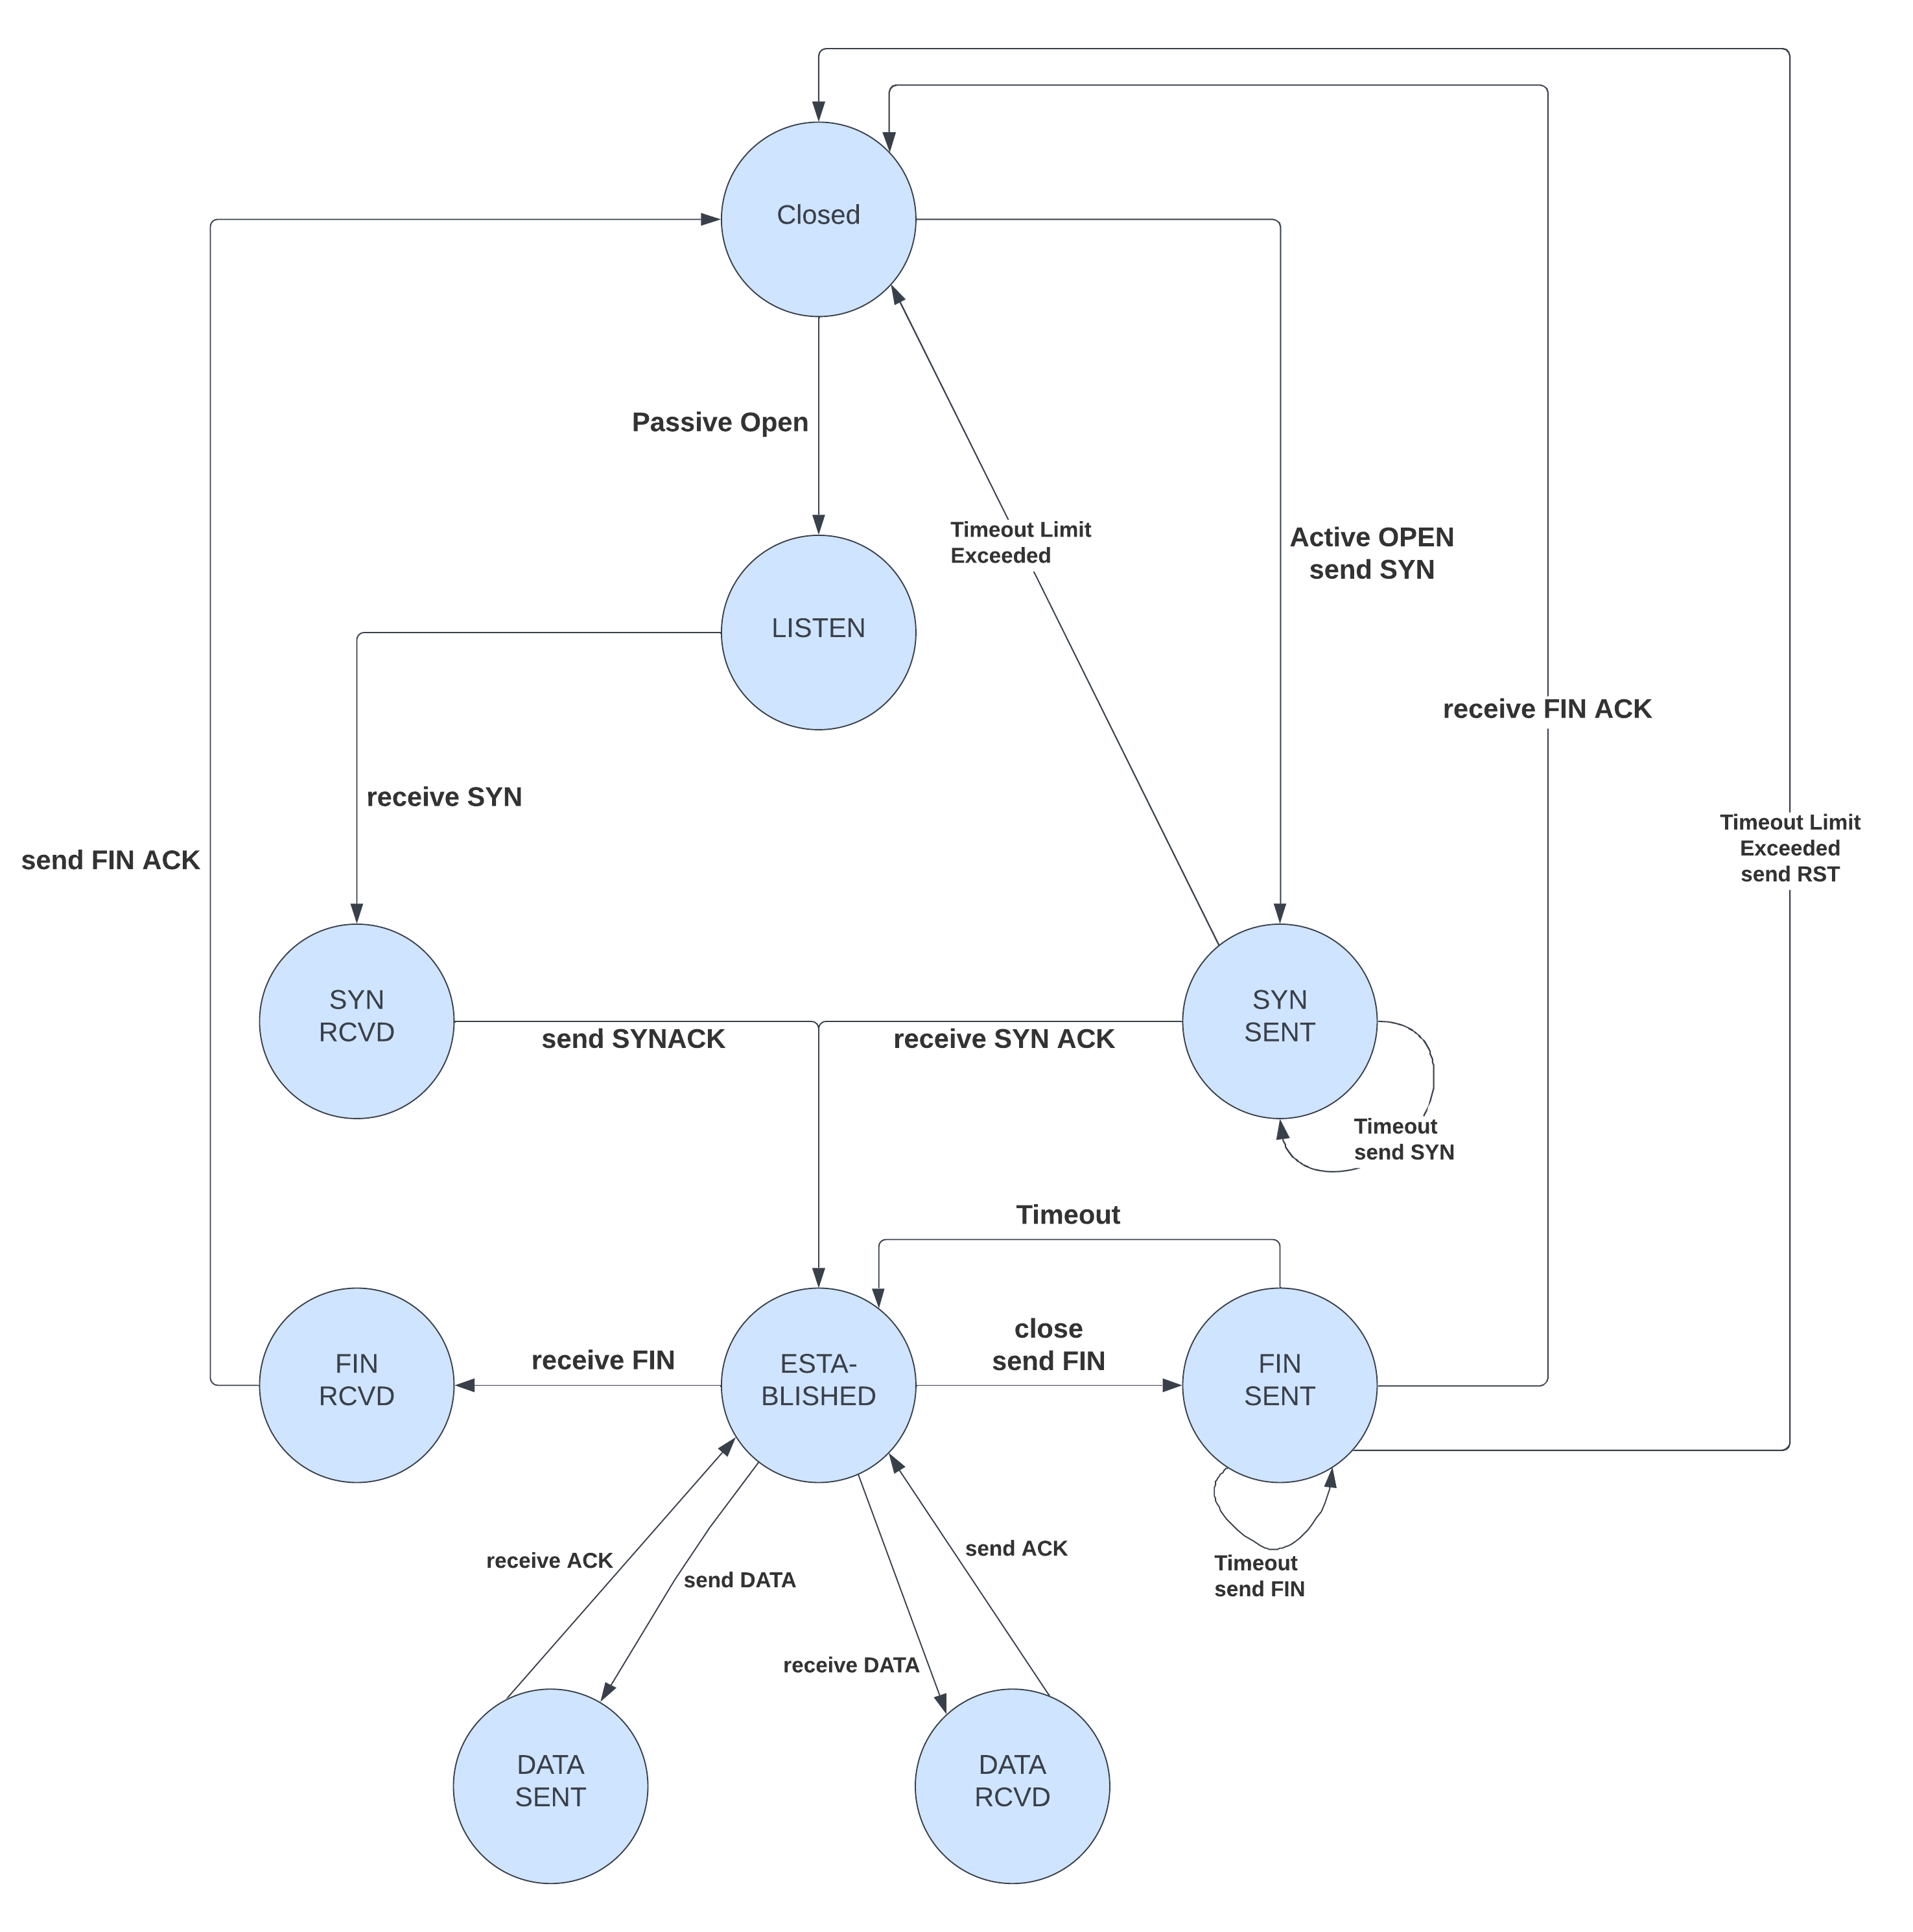
\includegraphics[width=120mm]{images/fsm.png}
\end{center}
\caption{Finite State Machine}\label{fig:fsm}
\end{figure}

\subsection{Connection Management}



200 ms is used initially for the handshake RTO, as packet is only 12 bytes.

Server timeouts not required.

\section{Testing}

This section will detail how RDT was tested to validate correct operation.

\subsection{Methodology}

To test the ability of RDT to deliver packets in a reliable and ordered manner, two test programs were created. The latter was run on \textbf{pc} and the former on \textbf{pc}. Slurpe was place in the middle. A file was transmitted from A to B. Decoded with SHA.


\section{Analysis}

\subsection{Performance in Different Network Scenarios}
\label{sec:performance}

\begin{figure}[H]
\begin{center}
    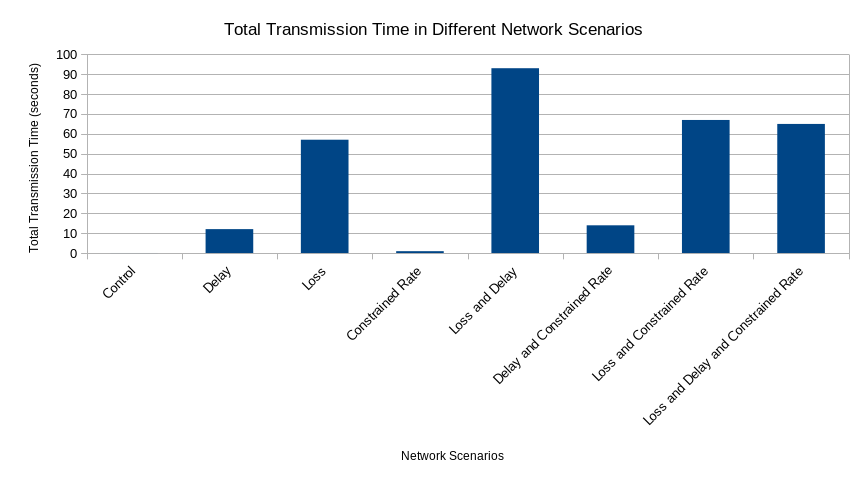
\includegraphics[width=100mm]{images/performance-network-scenarios.png}
\end{center}
\caption{Total Transmission Time in Different Network Scenarios for 230 Kb file.}\label{fig:performance}
\end{figure}

From Figure \ref{fig:performance} we can see that the network characteristic that has the biggest impact on the performance RDT is packet loss. 

\subsection{Bandwidth Delay Product and Link Utilisation}

The Bandwith-Delay Product (BDP) for a link represents the \textbf{what?} and is calculated as:

\begin{align*}
    BDP = \text{Bandwidth (bits per second)} \times \text{Round Trip Time (seconds)}
\end{align*}

For the link between \textbf{pcs} the observed average RTT with RDT was \textbf{RTT average}. This therefore yields a BDP of \textbf{BDP}.

As RDT only sends $1300 \text{\;bytes} = 10400 \text{\;bits}$ in each packet, this means that RDT achieves a link utilisation of $1040 / BDP = $.

\subsection{Maximum Theoretical Data Rate}



\subsection{Idle-RQ Performance}

\begin{align*}
    U_{RDT_IRQ} = \frac{N_pT_x}{T_x + 2T_p}
\end{align*}

where:
\begin{itemize}
    \item $N_p$ is the number of packets sent
    \item $T_x$ is the tranmission delay
    \item $T_p$ is the propogation delay
\end{itemize}

\subsection{RDT Packet Data Size}


\subsection{Wastage due to Control Information}

\begin{align*}
    \rho = \frac{i - c}{i + a} = \frac{1312 - 12}{1312 + 12} = 0.982 \text{\:(3 s.f.)}
\end{align*}

\end{document}